\documentclass[parskip=full]{scrartcl}
\usepackage[utf8]{inputenc} % use utf8 file encoding for TeX sources
\usepackage[T1]{fontenc}    % avoid garbled Unicode text in pdf
\usepackage[english]{babel}  % german hyphenation, quotes, etc
%\usepackage{bookmark}       % http://ctan.org/pkg/bookmark % fix has been ref. but does not exist error
\usepackage{graphicx}       % provides commands for including figures
\usepackage{csquotes}       % provides \enquote{} macro for "quotes"
\usepackage[nonumberlist]{glossaries}     % provides glossary commands
\usepackage{enumitem}
\usepackage{setspace}
\usepackage{subfigure}
\usepackage{pgf}
\usepackage{hyperref}       % detailed hyperlink/pdf configuration %should be loaded as last package
\setcounter{tocdepth}{2}
 
\makenoidxglossaries

\newglossaryentry{nn}
{
	name={neural network},
	description={A network or a circuit of neurons used for information processing inspired by the way biological neural systems process data.},
	plural={neural networks}
}

\newglossaryentry{img}
{
	name={image},
	description={A two dimensional matrix of red,green,blue (RGB) values that can be visualized as each cell represents a single pixel on the monitor. (ex.: a photo).},
	plural={images}
}

\newglossaryentry{cpu}
{
	name={CPU},
	description={Central Processing Unit},
	plural={CPUs}
}

\newglossaryentry{fpga}
{
	name={FPGA},
	description={Field Programmable Gate Array},
	plural={FPGAs}
}

\newglossaryentry{gpu}
{
	name={GPU},
	description={Graphics Processing Unit},
	plural={GPUs}
}

\newglossaryentry{json}
{
	name={JSON},
	description={JavaScript Object Notation}
}

\newglossaryentry{xml}
{
	name={XML},
	description={Extensible Markup Language}
}

\newglossaryentry{dp}
{
	name={deployment platform},
	plural={deployment platforms},
	description={Hardware to run the calculations on. (ex.: FPGA or CPU)}
}

\newglossaryentry{image classification}
{
	name={image classification},
	description={An object that is shown in a given picture is matched to a fitting class.}
}

\newglossaryentry{power consumption}
{
	name={power consumption},
	description={The power used per second by the system in Watts.}
}

\newglossaryentry{host pc}
{
	name={host pc},
	description={The main computer that is interacted with and used for input and output.}
}

\newglossaryentry{bb}
{
	name={bounding box},
	plural={bounding boxes},
	description={Rectangle indicating the outer edges of an object in an image.}
}

\newglossaryentry{performance}
{
	name={performance},
	description={Performance is the combination of the amount of \gls{flops} and the bandwidth.}
}

\newglossaryentry{ic}
{
	name={image class},
	plural={image classes},
	description={A class of the dataset on which the neural network is trained.}
}

\newglossaryentry{flops}{
	name={FLOPs},
	description={Floating Point Operations Per Second}
}

\newglossaryentry{bw}{
	name={bandwidth},
	description={The speed at which the data is transfered.}
}

\newglossaryentry{om}{
	name={operating mode},
	description={Description the performance and power consumption used for calculations.}
}

\newglossaryentry{binarisation}
{
	name={binarisation},
	description={Replaces float values by bool values (0 or 1). Drastically reduces the size of neural network and improves the running time. Reduces network accuracy.},
}

\newglossaryentry{prunning}
{
	name={prunning},
	description={Removes the neurons from the network, which have the lowest impact to the final result. Reduces the size of neural network and improves the running time. Reduces network accuracy.},
}

\title{Specifications}
\author{}

\begin{document}
\renewcommand{\figurename}{Figure}
\begin{titlepage}
\centering
	\vspace{3cm}
	{\scshape\LARGE Praxis der Softwarentwicklung\par}
	\vspace{2cm}
	{\scshape\Huge\bfseries Specificationsbook \par}	
	\vspace{2cm}
	{\scshape\Huge\bfseries Neural Network based Image Classification System on Heterogeneous Platforms\par}
	\vspace{2cm}
	{\Large from \par}
	\vspace{0.25cm}
	{\Large Team 2\\Dimitrov, Drehwald, Guneshka, Häring, Stangel \par}
	\vfill
\end{titlepage}
\newpage
\tableofcontents
\newpage
\section{Introduction}
In todays world of globalisation and digitalisation, to keep up with the rapidly growing economy, one important challenge is the automatisation of tasks. One aspect of this is the classification of visual inputs. Whether it is to check for broken parts in production or surveillance of public places. With the rapidly growing power of computers, \glspl{nn} are becoming more popular for tasks like this, as they need a lot of computational power but deliver sufficiently accurate results.\\
In the following project we want to build a framework with an intuitive graphical user interface to achieve these kinds of tasks.\\
To speed up the process of classification the software will be able to use different hardware that is more efficient for specific calculations. To further adjust the \gls{nn} to its task it should have different \glspl{om} to function on. High \gls{performance}, low \gls{power consumption} and a high energy effiency mode.


\section{Goal}
The goal of this project is to create a software which performs sufficiently accurate \gls{image classification} and is able to switch between \glspl{dp} and \glspl{om}. The software will be able to predict the \gls{power consumption} and the \gls{performance} (\gls{bw}, \gls{flops}).\\
The software should also have a GUI to interact with the program and to visualise the results.\\
The software should be extendable for further tasks.


\section{Product use}
The target group are engineers with a basic knowledge of data science.\\
The software is used to classify images on different \glspl{dp} with different \glspl{om} using a pretrained \gls{nn}.\\
Additionally, the software can be extended to be used for image detection, classification of frames from a videostream and training of a \gls{nn}.


\section{Criteria}
\subsection{Must Acceptance criteria}
\begin{tabular}{p{2cm}p{11.4cm}}
\textbf{MAC010} \hypertarget{MAC010} & \textbf{Image classification} \\
& The software can take a single image as input and returns the possiblities for each predefined \gls{ic}. The prediction is based on a pretrained \gls{nn}.\\
& \\
\textbf{MAC020} \hypertarget{MAC020} & \textbf{Running \gls{nn} on heterogeneous platforms} \\
& The software is able to communicate with \gls{cpu} and \gls{fpga}. The software is able to offload calculations to the different \glspl{dp} and receive the results.\\
& \\
\textbf{MAC030} \hypertarget{MAC030} & \textbf{Different \glspl{om}} \\
& The software has three \glspl{om}. One mode for high perfomance, one for low \gls{power consumption} and one for high energy efficiency. \\
& \\
\textbf{MAC040} \hypertarget{MAC040} & \textbf{Performance and \gls{power consumption} prediction}\\
& The software can predict the \gls{performance} with a certain \gls{power consumption} and also the \gls{power consumption} for a certain \gls{performance}.\\
& \\
\textbf{MAC050} \hypertarget{MAC050} & \textbf{GUI for interacting with software} \\
& The user is able to access the entire functionality described in \hyperlink{MAC010}{MAC010}-\hyperlink{MAC040}{MAC040} just by using the GUI. No coding or command line usage is required.
\end{tabular}

\subsection{Can Acceptance criteria}
\begin{tabular}{p{2cm}p{11.4cm}}
\textbf{CAC070} \hypertarget{CAC070} & \textbf{Illustration of the topology of a \gls{nn}} \\
& The software is able to visualise the topology of a given \gls{nn} (see figure 9). \\
\textbf{CAC071} \hypertarget{CAC071} & \textbf{The visualised \gls{nn} can be saved}\\
& The visualized \gls{nn} is saved as a .png file in a chosen directory.\\
& \\
\textbf{CAC080} \hypertarget{CAC080} & \textbf{Object Detection} \\
& The software can detect the \gls{bb} of an object. \\ 
& \\
\textbf{CAC090} \hypertarget{CAC090} &  \textbf{Using different models}\\
& The user is able to use different pretrained \glspl{nn} before an \gls{image classification} process. \\
& \\
\textbf{CAC100} \hypertarget{CAC100} & \textbf{Training \glspl{nn}} \\
& The software allows the user to train a \gls{nn} based on an predefined architecture.\\
& Neural networks trained by the user will be executed the same way \glspl{nn} provided with the software are executed.\\
& \\
\textbf{CAC110} \hypertarget{CAC110} & \textbf{Voting of multiple \glspl{nn}} \\
& The user is able to choose multiple \glspl{nn} for classification.\\
& The software will then execute all selected \glspl{nn} sequentially. The result presented to the user will be based on the weighted results of the different \glspl{nn}.\\
& \\
\textbf{CAC120} \hypertarget{CAC120} & \textbf{Using video for classification} \\
& The software is able to take a video, divide it into a certain amount of frames and perform \gls{image classification} for each frame.\\
& The classified frames are shown and can be iterated by the user. \\
& \\
\textbf{CAC130} \hypertarget{CAC130} & \textbf{Using camera for classification as input} \\
& The software takes the current frame from the camera connected to the \gls{host pc}, classifies it, displays the results and then when ready, takes the next available frame.\\
& \\
\textbf{CAC140} \hypertarget{CAC140} & \textbf{Running \gls{nn} on \gls{gpu}}\\
& \hyperlink{MAC020}{MAC020} is extended by \gls{gpu}.\\
\end{tabular}
\newpage
\begin{tabular}{p{2cm}p{11.4cm}}
\textbf{CAC150} \hypertarget{CAC150} & \textbf{Dropdown Menu for input mode selection}\\
& The software allows the user to select his preferred image input method using a dropdown menu.\\
& The dropdown menu entries are: \glqq Single Image\grqq, \glqq Folder\grqq, \glqq Camera\grqq, \glqq .txt file with \gls{img} paths\grqq.\\
& \\
\textbf{CAC160} \hypertarget{CAC160} & \textbf{Output parameter \glqq save all results\grqq}\\
& The software allows the user to select if the classification/detection output of each processed image should automatically be saved.\\
& \\
\textbf{CAC170} \hypertarget{CAC170} & \textbf{Output parameter \glqq show all results \grqq}\\
& The software allows the user to select if the software should wait for a user input after each image.\\
& If selected, the classification/ detection output for an image will be shown and the user has to click a button to continue with the next image.\\
& If not choosen, all selected images should be processed in the background and detached from the gui.\\
\end{tabular}

\subsection{Criteria of demarcation}
\begin{tabular}{p{2cm}p{11.4cm}}
\textbf{D010} & \textbf{No low-level optimization}\\
& Optimisations to reduce the execution time of object classification and detection will  be carried out in OpenCL.\\
& No optimizations including low-level languages or assembly intrinsics will be implemented.\\
&\\
\textbf{D020} & \textbf{No real time requirements}\\
& The software doesn't have to react in realtime. \\
& Code optimizations will be done in OpenCL to reduce the running time of the network per \gls{image classification}/ detection task.\\
&\\
\textbf{D030} & \textbf{No \gls{nn} size optimization}\\
& No techniques for memory usage reduction like \gls{prunning} or \gls{binarisation} will be implemented.\\
&\\
\textbf{D040} & \textbf{No mobile support}\\
& The software does not support mobile devices, like smartphones or wearables.\\
& \\
\textbf{D050} & \textbf{No input from commandline}\\
& The software does not support commandline input. The features are only useable with the GUI.
\end{tabular}

\section{Product environment}
The software runs on a computer in the lab at the CDNC institute. It has a CPU and an external FPGA connected via USB. Additionally, there is a \gls{gpu}.\\ 
The operating system is XUbuntu 18.04.


\section{Product data}
\begin{tabular}{p{2cm}p{11.4cm}}
\textbf{PD010} \hypertarget{PD010}& \textbf{Images for classification}\\
& The user can choose images of the format .jpg, .png, .bmp. The images are chosen by the user with the file explorer.\\
& \\
\textbf{PD020} \hypertarget{PD020} & \textbf{Config/weight file of pretrained model}\\
& The config file is a .cfg file with four sections, separated by <section>:\\
& In the first the classnames are given, one per line.\\
& In the second hyperparameters are described as \textit{<name> = <value>}. \\
& In the third layers are described in their order with the following format \textit{\lbrack kind of layer\rbrack}, 
each followed by a list of layer-parameters in the format \textit{<name> = <value>}\\
& In the last section the weights and biases for each layer are listed.\\
& \\
\textbf{PD030}\hypertarget{PD030} & \textbf{Labeled image set for classification training}\\
& The dataset is chosen by the user. The dataset is a directory with images and each image name has the format \\
& \textit{<id of image>\_<image class>}.\\
&\\
\textbf{PD040}\hypertarget{PD040} & \textbf{Labeled set of images for object detection training}\\
& It is a .txt file in the same directory as the images. The images are labeled with their name. The bounding box for each image are described in the .txt file with the same name as the image, in the format \textit{image class, x, y, width, height}. (X,Y) are the coordinates of the left bottom corner. (X, Y), width and height are relative. \\
& \\
\textbf{PD050}\hypertarget{PD050} & \textbf{Output format of image classification results if saved}\\
& If stored, the classification output will be saved in a <image name>.txt file. The format is \textit{<image class name> = <prohability>}, one row for each image class.\\
& If multiple images are processed, multiple .txt files will be created.\\
& \\
\textbf{PD060}\hypertarget{PD060} & \textbf{Output format of image detection results if saved}\\
& If stored, the detection output will be saved in a <image name>.txt file. The format is \textit{<image class name> = <prohability>, <X>, <Y>, <width>, <height>}, one row for each detected object.\\
& If multiple images are processed, multiple .txt files will be created.\\
& \\
\textbf{PD070\hypertarget{PD070}} & \textbf{Video input}\\
& The input video is in a .avi format.
\end{tabular}
\newpage
\section{Functional requirements}
\subsection{Image classification}
\subsubsection{Must}
\begin{tabular}{p{2cm}p{11.4cm}}
\textbf{MFR010}\hypertarget{MFR010} & \textbf{Use \gls{nn} for \gls{img} classification}\\
& Tested with: \hyperlink{T010}{T010} Implements: \hyperlink{MAC010}{MAC010} MAC010 \\                                    
& A \gls{nn} is used to classify \glspl{img}. The result is a list of prohabilities per image class.\\
\textbf{MFR011}\hypertarget{MFR011} & \textbf{Deploy pre-trained \gls{nn} with the corresponding layers}\\
& Tested with: \hyperlink{T011}{T011} Implements: \hyperlink{MAC010}{MAC010} \\
& A pre-trained \gls{nn} is deployed with its layers to a specified platform. The deployed \gls{nn} is used for MFR010.\\
\textbf{MFR012} \hypertarget{MFR012}& \textbf{Reading and parsing a \gls{nn} configuration/weight file}\\
& Tested with: \hyperlink{T012}{T012} Implements: \hyperlink{MAC010}{MAC010} \\
& The software is able to read a configuration file of a \gls{nn} and parse it for MFR011.\\
& \\
\end{tabular}
\subsubsection{Can}
\begin{tabular}{p{2cm}p{11.4cm}}
\textbf{CFR170} \hypertarget{CFR170} & \textbf{Voting of multiple \glspl{nn}}\\
& Tested with: \hyperlink{T170}{T170} Implements: \hyperlink{CAC110}{CAC110} \\
& The user can choose multiple \glspl{nn}. The \gls{image classification} is done on every \gls{nn} seperately and the results are weighted and accumulated.\\
\end{tabular}


\subsection{Operating modes}
\subsubsection{Must}
\begin{tabular}{p{2cm}p{11.4cm}}
\textbf{MFR020} \hypertarget{MFR020} & \textbf{High \gls{performance} \gls{om}}\\         
& Tested with: \hyperlink{T020}{T020} Implements: \hyperlink{MAC030}{MAC030} \\                           
& An \gls{om} to perform calculations as fast as possible.\\
\textbf{MFR021} \hypertarget{MFR021}& \textbf{Low \gls{power consumption} \gls{om}}\\ 
& Tested with: \hyperlink{T021}{T021} Implements: \hyperlink{MAC030}{MAC030} \\                                   
& An \gls{om} to perform calculations with low \gls{power consumption}.\\
\textbf{MFR022} \hypertarget{MFR022}& \textbf{Have high energy efficiency \gls{om}}\\      
& Tested with: \hyperlink{T022}{T022}  Implements: \hyperlink{MAC030}{MAC030} MAC030 \\                              
& An \gls{om} to perform calculations at an optimal ratio between \gls{performance} and \gls{power consumption}.\\
\textbf{MFR023}\hypertarget{MFR023} & \textbf{Calculator for \gls{power consumption}}\\ & Tested with: \hyperlink{T023}{T023} Implements:  \hyperlink{MAC040}{MAC040} \\                                   
& The software can calculate the \gls{power consumption} on a given \gls{nn}, \gls{om} and \gls{dp}.\\
\textbf{MFR024}\hypertarget{MFR024} & \textbf{Calculator for \gls{performance}}\\
& Tested with: \hyperlink{T024}{T024} Implements: \hyperlink{MAC040}{MAC040} \\                                    
& The software can calculate the \gls{performance} on a given \gls{nn}, \gls{om} and \gls{dp}.\\
\textbf {MFR025} \hypertarget{MFR025}& \textbf{Dispatching the calculation process defined from the \gls{om}}\\
& Tested with: \hyperlink{T020}{T020}, \hyperlink{T021}{T021}, \hyperlink{T021}{T021} Implements: \hyperlink{MAC030}{MAC030}\\
& The software is able to control the clock rate of the processor according to chosen \gls{om}. \\
\end{tabular}

\subsection{Platforms}
\subsubsection{Must}
\begin{tabular}{p{2cm}p{11.4cm}}
\textbf {MFR030}\hypertarget{MFR030} & \textbf{Support CPU for calculation} \\
& Tested with: \hyperlink{T030}{T030} Implements: \hyperlink{MAC020}{MAC020} \\
& The software supports CPU for calculation. \\
& \\
\textbf {MFR031}\hypertarget{MFR031}  & \textbf{Support FPGA for calculation} \\
& Tested with: \hyperlink{T031}{T031} Implements: \hyperlink{MAC020}{MAC020} \\
& The software supports FPGA for calculation. \\
& \\
\textbf {MFR040} \hypertarget{MFR040}& \textbf{Send image for classification} \\
& Tested with: \hyperlink{T040}{T040} Implements: \hyperlink{MAC020}{MAC020} \\
& The software gives the image as input for the \gls{nn} to the chosen \gls{dp}. \\
& \\
\textbf {MFR041} \hypertarget{MFR041}& \textbf{Receive result} \\
& Tested with: \hyperlink{T041}{T041} Implements: \hyperlink{MAC020}{MAC020} \\
& The program should be able to receive results of the executed \gls{image classification} from the \glspl{dp}. \\
& The software gives the image as input for the {nn} to the chosen \gls{dp}. \\
& \\
\end{tabular}
\subsubsection{Can}
\begin{tabular}{p{2cm}p{11.4cm}}
\textbf {CFR160} \hypertarget{CFR160} & \textbf{Support \gls{gpu} for calculation} \\
& Tested with: \hyperlink{T160}{T160} Implements: \hyperlink{CAC140}{CAC140} \\
& To speed up the calculations the program is able to use an additional \gls{gpu}.\\
& \\
\end{tabular}

\subsection{GUI}
\subsubsection{Must}
\begin{tabular}{p{2cm}p{11.4cm}}
\textbf {MFR050} \hypertarget{MFR050}& \textbf{GUI} \\
& Tested with: \hyperlink{T050}{T050} Implements: \hyperlink{MAC050}{MAC050} \\
& The program has a Graphical User Interface to display all functions to the user. \\
& \\
\textbf {MFR060}\hypertarget{MFR060}  & \textbf{Showing results} \\
& Tested with: \hyperlink{T060}{T060} Implements: \hyperlink{MAC050}{MAC050} \\
& After executing the \gls{image classification}, the results are shown in a bar chart. \\
& \\
\textbf{MFR070} \hypertarget{MFR070}& \textbf{Choosing image for classification}\\
& Tested with: \hyperlink{T070}{T070} Implements: \hyperlink{MAC050}{MAC050} \\
& The GUI has a button with an on click event which opens a file explorer. The explorer filters the files that only files of the format .jpg, .png, .bmp are listed.\\
& \\
\textbf{MFR080} \hypertarget{MFR080}& \textbf{Choosing \gls{dp}}\\
& Tested with: \hyperlink{T080}{T080} Implements: \hyperlink{MAC050}{MAC050} \\
& The GUI has a dropdown which lists the devices which are supported. The devices which can be theoretically be accessed but are not connected to the \gls{host pc} or the communication with them does not work are grayed out and not clickable. \\
& \\
\textbf{MFR090}\hypertarget{MFR090} & \textbf{Choosing \gls{om}}\\
& Tested with: \hyperlink{T090}{T090} Implements: \hyperlink{MAC050}{MAC050}  \\
& The GUI has dropdown which lists the different modes (high \gls{performance} mode, low \gls{power consumption} mode and high energy effiency mode). The \gls{power consumption} in Watts and \gls{performance} in \gls{flops} are also stated behind the operating mode names.
\end{tabular}
\subsubsection{Can}
\begin{tabular}{p{2cm}p{11.4cm}}
\textbf{CFR100} \hypertarget{CFR100} & \textbf{Choosing between different \glspl{nn}}\\
& Tested with: \hyperlink{T100}{T100} Implements: \hyperlink{CAC090}{CAC090} \\
& The GUI has a button which opens the file explorer which filters for .cfg files. There you choose the config file of the \gls{nn} which you want to use. The program loads this config and parses it so it can be deployed. Possible models would be GoogLeNet or AlexNet.\\
& \\
\textbf {CFR112} \hypertarget{CFR112} & \textbf{Choosing and loading data set} \\
& Tested with: \hyperlink{T112}{T112} Implements: \hyperlink{CAC100}{CAC100}\\
& The software has an option to select a set of labeled images and for loading those.\\
\textbf {CFR114} \hypertarget{CFR114} & \textbf{Change the learning rate} \\
& Tested with: \hyperlink{T114}{T114} Implements: \hyperlink{CAC100}{CAC100} \\
& To adjust the learning proccess of the \gls{nn} the user can change the speed of how fast the weights and biases will be changed with a textbox. Only floats are valid.\\
& \\
\textbf {CFR120} \hypertarget{CFR120} & \textbf{Visualisiaton of \gls{nn}} \\
& Tested with: \hyperlink{T120}{T120} Implements: \hyperlink{CAC070}{CAC070} \\
& The software is able to visualise the topology of a \glspl{nn} (see figure 9) \\
\textbf{CFR121} \hypertarget{CFR121} & \textbf{Saving the visualisation}\\
& Tested with: \hyperlink{T121}{T121} Implements: \hyperlink{CAC071}{CAC071} \\
& The user can save the visualition of the topology of a \gls{nn} as .png file to a chosen directory.\\
& \\
\textbf {CFR131} \hypertarget{CFR131} & \textbf{Showing detected object} \\
& Tested with: \hyperlink{T131}{T131} Implements: \hyperlink{CAC080}{CAC080}\\
& The found objects are marked by a \gls{bb}. The \gls{bb} is drawn on the image. This picture is shown.\\
& \\
\textbf{CFR140} \hypertarget{CFR140} & \textbf{Choosing and loading video}\\
& Tested with: \hyperlink{T140}{T140} Implements: \hyperlink{CAC120}{CAC120} CAC120 \\
& The user can choose a video and the software can use it as input for the classification/detection process.\\
\end{tabular}
\newpage
\begin{tabular}{p{2cm}p{11.4cm}}
\textbf{CFR180} \hypertarget{CFR180} & \textbf{Dropdown menu for input selection}\\
& Tested with: \hyperlink{T180}{T180} Implements: \hyperlink{CAC160}{CAC160} \\
& A dropdown menu is part of the classification and detection page.\\
& It contains the four options: Single Image, Image folder, Camera, .txt File with Img Paths\\
& Single \gls{img} is \hyperlink{MFR070}{MFR070}\\
& Image folder opens the file explorer with the filter for directories. Images with a valid format are loaded from this directory.\\
& .txt File with \gls{img} paths opens the file explorer with filter for .txt files. \\
& Camera opens a connection to a connected camera and receives the video stream.\\
& \\
\textbf{CFR190} \hypertarget{CFR190} & \textbf{Selector for output parameter \glqq save all results\grqq}\\
& Tested with: \hyperlink{T190}{T190} Implements: \hyperlink{CAC160}{CAC160} \\
& A checkbox is part of the classification and detection page.\\
& If selected, for each image which has been selected by the user, the classification/ detection output will be stored as described in PD050 and PD060. Each output file is saved in the same folder as the input file.\\
& If a camera is choosen as input, the output will be stored in a \glqq camera\grqq folder\\
& \\
\textbf{CFR200} \hypertarget{CFR200} & \textbf{Selector for output parameter \glqq show all images\grqq}\\
& Tested with: \hyperlink{T200}{T200} Implements:  \hyperlink{CAC170}{CAC170}\\
& If selected, the output for each image processed will be shown as described in CFR131 and MFR060.\\
& The user has to manually select \glqq continue\grqq  before the software will continue with processing the next image.\\
& If not selected, all images choosen by the user will be processed continuesly without showing classification/ detection output in the GUI.\\
\end{tabular}

\subsection{Training}
\subsubsection{Can}
\begin{tabular}{p{2cm}p{11.4cm}}
\textbf{CFR110} \hypertarget{CFR110} & \textbf{Train \gls{nn} for classification of imageset}\\
& Tested with: \hyperlink{T110}{T110} Implements: \hyperlink{CAC100}{CAC100} \\
& The user chooses a \gls{nn} and a new imageset and trains the \gls{nn} on this new imageset. If it is pretrained it uses transfer learning with the existing weights otherwise random values.\\
\textbf {CFR111} \hypertarget{CFR111} & \textbf{Saving newly trained \gls{nn}} \\
& Tested with: \hyperlink{T111}{T111} Implements: \hyperlink{CAC100}{CAC100} \\
& The software is able to take the weights and config of an newly trained \glspl{nn} and save it as .cfg file. \\
\textbf {CFR113} \hypertarget{CFR113} & \textbf{Backpropagation} \\
& Tested with: \hyperlink{T113}{T113} Implements: \hyperlink{CAC100}{CAC100} \\
& The software is able to adjust the weights and biases of the \gls{nn} in the training process with backpropagation.\\
\textbf{CFR115} \hypertarget{CFR115} & \textbf{Fit the output layer to the amount of \glspl{ic}}\\
& Tested with: \hyperlink{T115}{T115} Implements: \hyperlink{CAC100}{CAC100} \\
& If the user trains a \gls{nn} with a dataset, the number of output nodes are adapted to the number of \glspl{ic}.\\
\end{tabular}

\subsection{Object detection}
\subsubsection{Can}
\begin{tabular}{p{2cm}p{11.4cm}}
\textbf {CFR130} \hypertarget{CFR130} & \textbf{Object detection} \\
& Tested with: \hyperlink{T130}{T130} Implements: \hyperlink{CAC080}{CAC080} \\
& The software can detect the position and \gls{ic} of objects in an image.\\

\end{tabular}

\subsection{Video handling}
\subsubsection{Can}
\begin{tabular}{p{2cm}p{11.4cm}}
\textbf{CFR150} \hypertarget{CFR150} & \textbf{Connect with camera}\\
& Tested with: \hyperlink{T150}{T150} Implements: \hyperlink{CAC130}{CAC130} \\
& The software can connect with a camera connected to the \gls{host pc}.\\
\textbf{CFR151} \hypertarget{CFR151} & \textbf{Receive video stream from camera}\\
& Tested with: \hyperlink{T151}{T151} Implements: \hyperlink{CAC130}{CAC130}\\
& The software can receive a video stream from the camera.\\
\textbf{CFR152} \hypertarget{CFR152} & \textbf{Apply classifcation/detection for a certain amount of frames}\\
& Tested with: \hyperlink{T152}{T152} Implements: \hyperlink{CAC130}{CAC130}\\
& The software can devide a video or videostream into frames and is able to apply \gls{image classification} and detection on those.\\
\textbf{CFR153} \hypertarget{CFR153} & \textbf{Saving the frames}\\
& Tested with: \hyperlink{T152}{T152} Implements: \hyperlink{CAC120}{CAC120}\\
& The software devides the video into frames which are saved to the file system.
\end{tabular}


\section{Non-functional requirements}
\begin{tabular}{p{2cm}p{11.4cm}}
\textbf{NFR010} & \textbf{Project size}\\
& The project should have around ten thousand (10,000) lines of code \\
& \\
\textbf{NFR020} & \textbf{Code size}\\
& The project should be done with Object-Orientated programming. The whole project should have around fourty (40) to eighty (80) classes excluding interfaces. \\
& \\
\textbf{NFR030} & \textbf{Model-View-Controller}\\
& The project should be based on the design pattern model-view-controller. \\
& \\
\textbf{NFR040} & \textbf{Programming language}\\
& The software is written in C++ and OpenCL.\\
& \\
& \\
\textbf{NFR050} & \textbf{Minimal size of training dataset}\\
& The software works with a dataset with a minimum of 100 images.
\end{tabular}


\section{Test cases}
\begin{tabular}{p{2cm}p{11.4cm}}
\textbf{T010} \hypertarget{T010} & \textbf{Use \gls{nn} for \gls{img} classification}\\
T010.1& \textbf{State:} An \gls{img} as input, a pretrained \gls{nn}, a \gls{dp} and an \gls{om} is given.\\
& \textbf{Action:} The user clicks on \glqq Start \gls{image classification}\grqq.\\
& \textbf{Reaction:} The image is classified by the \gls{nn} and results are shown.\\
& \\
\textbf{T011} \hypertarget{T011} & \textbf{Deploy pre-trained \gls{nn}}\\
T011.1 & \textbf{State:} The pretrained \gls{nn} is loaded and parsed.\\
& \textbf{Action:} The user clicks on \glqq Start \gls{image classification}\grqq.\\
& \textbf{Reaction:} The software loads the model to the \gls{dp}.\\
& \\
\textbf{T012} \hypertarget{T012} & \textbf{Reading and parsing \gls{nn} configuration file}\\
T012.1 & \textbf{State:} A .cfg file with the configuration of a pretrained \gls{nn} is given.\\
& \textbf{Action:} The user clicks on \glqq Start \gls{image classification}\grqq.\\
& \textbf{Reaction:} The software loads the model and parses it .\\
T012.2 & \textbf{State:} The file explorer is open\\
& \textbf{Action:} The user selects a \gls{nn} to import\\
& \textbf{Reaction:} The file explorer closes and the \gls{nn} is imported and selected for the classification.\\
& \\
\textbf{T020} \hypertarget{T020} & \textbf{High \gls{performance} \gls{om}}\\
T020.1 & \textbf{State:} An \gls{img} as input, a pretrained \gls{nn}, a \gls{dp} is given .\\
& \textbf{Action:} The user chooses to perform the calculations in high \gls{performance} \gls{om} and starts the classification.\\
& \textbf{Reaction:} The calculations run considerably faster than in the other possible modes with the same conditions.\\
& \\
\textbf{T021} \hypertarget{T021} & \textbf{Low \gls{power consumption} \gls{om}}\\
T021.1 & \textbf{State:} An \gls{img} as input, a pretrained \gls{nn}, a \gls{dp} is given.\\
& \textbf{Action:} The user chooses to perform the calculations in low \gls{power consumption} \gls{om} and starts the classification.\\
& \textbf{Reaction:} The calculations run with considerably lower \gls{power consumption} than with the other possible modes in the same conditions.\\
& \\
\end{tabular}
\newpage
\begin{tabular}{p{2cm}p{11.4cm}}
\textbf{T022} \hypertarget{T022} & \textbf{High energy efficiency \gls{om}}\\
T022.1 & \textbf{State:} An \gls{img} as input, a pretrained \gls{nn}, a \gls{dp} is given.\\
& \textbf{Action:} The user chooses to perform the calculations in high energy efficiency \gls{om} and starts the classification.\\
& \textbf{Reaction:} The calculations run with regard to balance between \gls{power consumption} and speed.\\
& \\
\textbf{T023} \hypertarget{T023} & \textbf{Calculator for \gls{power consumption}}\\
T022.1 & \textbf{State:} A pretrained \gls{nn}, a \gls{dp}  and the \gls{om} is given.\\
& \textbf{Action:} The user chooses another \gls{om}.\\
& \textbf{Reaction:} The new \gls{power consumption} is calculated automatically and then shown.\\
& \\
\textbf{T024} \hypertarget{T024} & \textbf{Calculator for \gls{performance}}\\
T022.1 & \textbf{State:} A pretrained \gls{nn}, a \gls{dp}  and the \gls{om} is given.\\
& \textbf{Action:} The user chooses another \gls{om}.\\
& \textbf{Reaction:} The new \gls{performance} is calculated automatically and then shown.\\
& \\
\textbf{T030} \hypertarget{T030} & \textbf{Support CPU for calculation} \\
T030.1 & \textbf{State:} An \gls{img} as input, a pretrained \gls{nn}, CPU as \gls{dp} and an \gls{om} is given. \\
& \textbf{Action:} Click on the button \glqq Start \gls{image classification}\grqq \\
& \textbf{Reaction:} Elephant has the highest probability. \\
& \\
\textbf{T031} \hypertarget{T031} & \textbf{Support FPGA for calculation} \\
T031.1 & \textbf{State:} An \gls{img} as input, a pretrained \gls{nn}, FPGA as \gls{dp} and an \gls{om} is given. \\
& \textbf{Action:} Click on the button \glqq Start \gls{image classification}\grqq \\
& \textbf{Reaction:} Elephant has the highest probability. \\
& \\
\textbf{T040} \hypertarget{T040} & \textbf{Send image for classification} \\
T040.1 & \textbf{State:} An \gls{img} as input, a pretrained \gls{nn}, a \gls{dp} and an \gls{om} is given. \\
& \textbf{Action:} The user starts \gls{image classification}  \\
& \textbf{Reaction:} The software sends the image as array to the selected platform.\\
\end{tabular}
\newpage
\begin{tabular}{p{2cm}p{11.4cm}}
\textbf{T041} \hypertarget{T041} & \textbf{Receive result}\\
T041.1 & \textbf{State:} The software is awaiting result. \\
& \textbf{Action:} Platform sends results. \\
& \textbf{Reaction:} The software receives the results from the platform and shows it. \\
& \\
\textbf{T050} \hypertarget{T050} & \textbf{GUI} \\
T050.1 & \textbf{State:} The user wants to use the software.\\
& \textbf{Action:} The user starts the program. \\
& \textbf{Reaction:} The users sees the Graphical User Interface showed on \\
& Figure 1. \\
& \\
\textbf{T060} \hypertarget{T060} & \textbf{Showing results} \\
T060.1 & \textbf{State:} The software awaits result. \\
& \textbf{Action:} The \gls{dp} sends result.\\
& \textbf{Reaction:} The Graphical User Interface shows the result in a bar chart as shown in figure 4. \\
& \\
\textbf{T070} \hypertarget{T070} & \textbf{Choosing image for classification}\\
T070.1 & \textbf{State:} The user is on the page for \gls{image classification}. \\
& \textbf{Action:} The user clicks on the button \glqq Choose image\grqq.\\
& \textbf{Reaction:} The file explorer opens with the filter for .png, .jpg, .bmp.\\
T070.2 & \textbf{State:} The file explorer is open.\\
& \textbf{Action:} The user selects an image with a valid format.\\
& \textbf{Reaction:} The file explorer closes and image is loaded and shown as preview.\\
& \\
\textbf{T080} \hypertarget{T080} & \textbf{Choosing platform/hardware}\\
T080.1 & \textbf{State:} The user is on the page for \gls{image classification}.\\
& \textbf{Action:} The user chooses the desired \gls{dp} with the dropdown.\\
& \textbf{Reaction:} An internal flag is set to the desired platform and the dropdown shows the chosen \gls{dp}.\\
& \\
\textbf{T090} \hypertarget{T090} & \textbf{Choosing \gls{om}}\\
T090.1 & \textbf{State:} The user is on the page for \gls{image classification}.\\
& \textbf{Action:} The user chooses the desired \gls{om} with the dropdown.\\
& \textbf{Reaction:} An internal flag is set to the desired \gls{om} and the dropdown shows the chosen \gls{om}\\
& \\
\end{tabular}
\newpage
\begin{tabular}{p{2cm}p{11.4cm}}
\textbf{T100} \hypertarget{T100} & \textbf{Choosing between different \gls{nn}}\\
T100.1 & \textbf{State:} The user is on the page for \gls{image classification}.\\
& \textbf{Action:} The user clicks on the button \glqq Choose \gls{nn}\grqq.\\
& \textbf{Reaction:} The file explorer opens.\\
T100.2 & \textbf{State:} The file explorer is open.\\
& \textbf{Action:} The user selects a config file.\\
& \textbf{Reaction:} The file explorer closes and the software loads the input and parses it. If it is loaded there is a success message shown.\\
& \\
\textbf{T110} \hypertarget{T110} & \textbf{Train \gls{nn} for classification of imageset}\\
T110.1 & \textbf{State:} The user is on the main page.\\
& \textbf{Action:} The user clicks the button \glqq Train a \gls{nn}\grqq.\\
& \textbf{Reaction:}The user is redirected to a new page for training, shown in figure 6.\\
T110.2 & \textbf{State:} The user is on the page for training, has selected a \gls{nn}, a dataset for training, the kind of training (backpropagation or transfer learning if possible), the learning rate and the desired precision.\\
& \textbf{Action:} The user clicks on the button \glqq Train\grqq\\
& \textbf{Reaction:} The software starts to train the selected \gls{nn} and shows the progress in a line graph.\\
T110.3 & \textbf{State:} The training is in process.\\
& \textbf{Action:} The precision reaches the desired precision.\\
& \textbf{Reaction:} The training stops.\\
& \\
\textbf{T111} \hypertarget{T111}& \textbf{Saving a \gls{nn} after training}\\
T111.1 & \textbf{State:} The training finishes.\\
& \textbf{Action:} No action required.\\
& \textbf{Reaction:} The software stores the trained \gls{nn} in the directory of the selected .cfg file as a .cfg file.\\
& \\
\textbf{T112} \hypertarget{T112} & \textbf{Choosing and reading dataset}\\
112.1 & \textbf{State:} The user is on the training page.\\
& \textbf{Action:} The user clicks on \glqq Choose dataset\grqq. \\
& \textbf{Reaction:} A file explorer opens.\\
T112.2 & \textbf{State:} The file explorer is open.\\
& \textbf{Action:} The user chooses the folder with the images. \\
& \textbf{Reaction:} The program automatically iterates over all images and reads the given data that can be used for training.\\
\end{tabular}
\newpage
\begin{tabular}{p{2cm}p{11.4cm}}
\textbf{T113} \hypertarget{T113}& \textbf{Backpropagation}\\
T113.1 & \textbf{State:} The user is on the training page, a dataset, a \gls{nn}, learning rate and desired precision are given.\\
& \textbf{Action:} The user clicks on \glqq Train\grqq.\\
& \textbf{Reaction:} The software adjusts the weights and biases of the corresponding \gls{nn} via backpropagation to improve its precision. These changes are then shown with a diagram.\\
&\\
\textbf{T114} \hypertarget{T114}& \textbf{Changing parameters}\\
T114.1 & \textbf{State:} The user chose a \gls{nn}, the dataset and the desired precision. \\
& \textbf{Action:} The user changes the learning rate to a smaller number and starts training. \\
& \textbf{Reaction:} The \gls{nn} adjusts its weights but with smaller significance of one image. \\
&\\
\textbf{T115} \hypertarget{T115}& \textbf{Fit the output layer to the maount of image classes}\\
T115.1 & \textbf{State:} The user chose a \gls{nn} with ten output nodes and a dataset with 12 image classes.\\
& \textbf{Action:} The user starts the training\\
& \textbf{Reaction:} The output layer is extended by two nodes as well as weights for the new connections are initilised. \\
& \\
\textbf{T120} \hypertarget{T120}& \textbf{Showing topology of a \gls{nn}}\\
T120.1 & \textbf{State:} The user is on the main page.\\
& \textbf{Action:} The user clicks the \glqq Show topology of a \gls{nn}\grqq button.\\
& \textbf{Reaction:} The user is redirected to a new page for showing a topology.\\
T120.2 & \textbf{State:} The user is on the page for showing the topology.\\
& \textbf{Action:} The user clicks on \glqq Choose topology to show\grqq\\
& \textbf{Reaction:} The file explore opens\\
T120.3 & \textbf{State:} The file explorer is open.\\
& \textbf{Action:} The user choses a .cfg file.\\
& \textbf{Reaction:} The file explorer closes and the topology is shown as in \\
& figure 9. \\
& \\
\textbf{T121} \hypertarget{T121}& \textbf{Saving topology visualisation}\\
T121.1 & \textbf{State:} The user is on the show topology page and a topology is shown.\\
& \textbf{Action:} The user clicks on the save button.\\
& \textbf{Reaction:} The visualisation is saved to the file system.\\
\end{tabular}
\newpage
\begin{tabular}{p{2cm}p{11.4cm}}
\textbf{T130} \hypertarget{T130}& \textbf{Object detection}\\
T130.1 & \textbf{State:} The detection window is open. An \gls{img} as input, a pretrained \gls{nn}, a \gls{dp} and an \gls{om} is given.\\
& \textbf{Action:} The user clicks on the button \glqq start detection\grqq\\
& \textbf{Reaction:} The network is run for inferencing and the network output is shown to the user.\\
& \\
\textbf{T131} \hypertarget{T131} & \textbf{Drawing \gls{bb}}\\
T131.1 & \textbf{State:} Inferencing was executed on an image given by the user, the choosen \gls{nn} predicted \glspl{bb}.\\
& \textbf{Action:} No action required\\
& \textbf{Reaction:} The original image, given by the user, is overlayed with the boxes predicted by the network, the updated image is presented to the user.\\
& \\
\textbf{T140} \hypertarget{T140} & \textbf{Choosing video}\\
T140.1 & \textbf{State:} The software is running. A pretrained \gls{nn}, a \gls{dp} and an \gls{om} is given. \\
& \textbf{Action:} The user selects a .avi video file.\\
& \textbf{Reaction:} The system stores the path to the selected video and is \\
& available to process images from this video sequentially.\\
& \\
\textbf{T150} \hypertarget{T150} & \textbf{Connect with camera}\\
T150.1 & \textbf{State:} The software is running.\\
& \textbf{Action:} The user connects a usb camera to the host.\\
& \textbf{Reaction:} The system dynamically detects the camera and allows the user to select the camera as an image source\\
T150.2 & \textbf{State:} A usb camera is connected to the host. The software is not running.\\
& \textbf{Action:} The user starts the software.\\
& \textbf{Reaction:} The system dynamically detects the camera and allows the user to select the camera as an image source\\
& \\
\textbf{T151} \hypertarget{T151} & \textbf{Receive video stream from camera}\\
T151.1 & \textbf{State:} The software is running, a camera is available as image source.\\
& \textbf{Action:} The user chooses the camera as image source.\\
& \textbf{Reaction:} The first camera image is provided as a preview, the continuous image stream is available for further processing.\\
\end{tabular}
\newpage
\begin{tabular}{p{2cm}p{11.4cm}}
\textbf{T152} \hypertarget{T152}& \textbf{Apply classification for a certain amount of frames}\\
T152.1 & \textbf{State:} The software is running. A video source was choosen by the user. All network details were provided by the user. Classification was choosen by the user.\\
& \textbf{Action:} The user clicks on the button \glqq start classification\grqq\\
& \textbf{Reaction:} The software devides the video into frames and saves them. The software sequentially classifies the pictures and outputs the result as set.\\
& \\
\textbf{T160} \hypertarget{T160}& \textbf{Support \gls{gpu} for classification}\\
& \textbf{State:} The classification window is open. An \gls{img} as input, a pretrained \gls{nn}, a \gls{dp} and an \gls{om} is given.\\
& \textbf{Action:} The user chooses \gls{gpu} as a \gls{dp}. The user clicks on the button \glqq Start \gls{image classification}\grqq \\
& \textbf{Reaction:} \gls{image classification} is performed on the gpu.\\
& \\
\textbf{T170} \hypertarget{T170} & \textbf{Voting of multiple \gls{nn}}\\
T170.1 & \textbf{State:} The user is on the classification page. He has chosen three different \glspl{nn}, one \gls{img}, a mode, a \gls{dp}.\\
& \textbf{Action:} The user clicks on the button \glqq start classification\grqq.\\
& \textbf{Reaction:} The software starts the calculations. When those finished, the software receives three lists of the result. Elephant has the highest prohability in any results list. It is shown as result.\\
& \\
\textbf{T180} \hypertarget{T180} & \textbf{Choosing Input Mode}\\
T180.1 & \textbf{State:} The classification window is open. \\
& \textbf{Action:} The user clicks on the dropdown Menu \glqq Input Mode\grqq\ and selects \glqq Single Image\grqq\\
& \textbf{Reaction:} The dropdown Menu shows the selection \glqq Single Image\grqq. The File explorer is set to show .jpg, .png and .bmp files\\
T180.2 & \textbf{State:} The detection window is open. \\
& \textbf{Action:} The user clicks on the dropdown Menu \glqq Input Mode\grqq\ and selects \glqq Image Folder\grqq\\
& \textbf{Reaction:} The dropdown Menu shows the selection \glqq Image Folder\grqq. The File explorer is set to show folders only.\\
T180.3 & \textbf{State:} The classification window is open. A Camera is connected to the Host PC\\
& \textbf{Action:} The user clicks on the dropdown Menu \glqq Input Mode\grqq\ and selects \glqq Camera\grqq\\
& \textbf{Reaction:} The dropdown Menu shows the selection \glqq Camera\grqq. The File explorer button is replaced by a text label saying \glqq Camera connected\grqq \\
\end{tabular}
\newpage
\begin{tabular}{p{2cm}p{11.4cm}}
T180.4 & \textbf{State:} The detection window is open. A Camera is not connected to the Host PC\\
& \textbf{Action:} The user clicks on the dropdown Menu \glqq Input Mode\grqq\ and selects \glqq Camera\grqq\\
& \textbf{Reaction:} The dropdown Menu shows the selection \glqq Camera\grqq. The File explorer button is replaced by a text label saying \glqq No camera connected\grqq \\
T180.5 & \textbf{State:} The classification window is open.\\
& \textbf{Action:} The user clicks on the dropdown Menu \glqq Input Mode\grqq\ and selects \glqq txt file with Image Paths\grqq\\
& \textbf{Reaction:} The dropdown Menu shows the selection \glqq txt file with Image Paths\grqq. The File explorer is set to show .txt files\\
& \\
\textbf{T190} \hypertarget{T190} & \textbf{Output Mode \glqq Save all results\grqq}\\
T190.1 & \textbf{State:} The classification window is open. Input Mode was set to \glqq Image Folder\grqq\ and a folder containing multiple .png images was selected. \glqq Save all results\grqq\ has been selected. All other Input parameters have been set.\\
& \textbf{Action:} The user clicks on \glqq start detection\grqq\\
& \textbf{Reaction:} The systems calculates the classification output for each image. The output is stored in one .txt file per image as described in \hyperlink{PD050}{PD050}\\
T190.2 & \textbf{State:} The detection window is open. Input Mode was set to \glqq txt file with Img Paths\glqq\ and a file containing multiple paths to .png images was selected. \glqq Save all results\grqq\ has been selected. All other Input parameters have been set.\\
& \textbf{Action:} The user clicks on \glqq start detection\grqq\\
& \textbf{Reaction:} The systems calculates the detection output for each image. The output is stored in one .txt file per image as described in \hyperlink{PD060}{PD060}\\
& \\
\textbf{T200} \hypertarget{T200}& \textbf{Show all results}\\
T200.1 & \textbf{State:} The user choosed to classify five \gls{img} and chose to show all results. The software awaits the results.\\
& \textbf{Action:} The software receives the results.\\
& \textbf{Reaction:} The first result and a continue button is shown.
\end{tabular}
\newpage
\section{System models}
\subsection{Scenarios}
\subsubsection{Scenario 1}
The user U1 wants to classify the image of a cat. He goes on the classifcation page and he clicks on the dropdown and sees the three \glspl{om} \glqq low \gls{power consumption}\grqq , \glqq high perfomance\grqq and \glqq high energy effiency\grqq . He can also see the predicted \gls{power consumption} and \gls{performance}. He chooses to classificate in the low power mode and runs the programm. The results are shown.
\subsubsection{Scenario 2}
The user U2 goes to the classification page and chooses the image of a coala and the high power \gls{performance} mode and CPU mode. The software states that it would take 86 watts with 166 G\gls{flops}. U2 decides he would rather use the high energy effiency mode with 140 G\gls{flops} and 70 watts. He sets the other parameters and clicks on Start \gls{image classification}. The result is that the image is a coala and shows this result. 
\subsubsection{Scenario 3}
The user U3 created the blueprint for a new \gls{nn} in .cfg.\\
She wants to train a network based on this config file but computation time is shared and expensive. Therefore U3 has to convince her boss.
U3 uses the software with her \gls{nn} as input and selects the visualisation toolkit.\\
U3 saves the output and uses it during the discussion to demonstrate the advantages of her new \gls{nn}.
\clearpage
\subsubsection{Scenario 4}
User U4 has to categorise a large dataset of plants from a biology field trip. U4 has two trained \glspl{nn} for this task. The first with a good accuracy and high confidence on leaves. The second with a high confidence and accuracy on flowers. On unknown objects they both tend to have a low confidence. U4 does not want to manually decide which network to use for every image. He also does not want to train a new \gls{nn}. Therefore U4 selects both networks and the folder with the new images inside, as well as the parameters save-result and dont-show results. The software classifies all images in a few minutes and he is able to handover the dataset for further documentation.
\subsubsection{Scenario 5}
User U5 has heared about this software and wants to test it.
U5 is a pokemon fan, therefore he decides to use a new \gls{nn} to classify the newest generation pokemon. None of the provided networks was trained for that task, so U5 decides to train a new \gls{nn}. U5 copies an existing \gls{nn} layout file and adds five (5) fully connected layers in between to create a larget \gls{nn}. U5 uses his large pokemon image dataset, his new \gls{nn} layout file and the software, to train a new \gls{nn}. 
Afterwards U5 creates a folder with new pokemon images and uses his new network and the software to classify them.
\subsubsection{Scenario 6}
U6 had a trip in Africa and made a lot of pictures of animals. He looks for an easy way to know how many different species of animals he saw and took photos of. Alex doesn't know how to code or to run a program thus he needs a friendly and understandable Graphical User Interface, that our software offers. Alex opens the main menu of the software where he sees that it's possible to finish his task, without any knowledge, because of the GUI. 
\clearpage
\subsubsection{Scenario 7}
U7, a company, wants to develop an AI to feed the animals at Zoos. The company does not have enough labelers to label all of the frames they need to teach the software which animal it is seeing at the moment. U7 decides to use the software for object detection. An employee goes on the Detection page of the software and uses it to label the frames required for the AI.
\subsubsection{Scenario 8}
The company U8 wants to teach small kids parallel to read, recognize percents and animals. The software is just right for the job, because of the \gls{image classification} option of the software. The CEO of U8 hears about Tucs and now wants to test it. He assigns a few employees with their kids to try the software. The results are outstanding! Because of the intuitive layout and the structure of the \gls{image classification} page of the software, the kids are able to learn and also having fun at the same time.
\clearpage
\subsection{Usecases}
\subsubsection{Image classification page}
\begin{figure}[htb!]
\centering
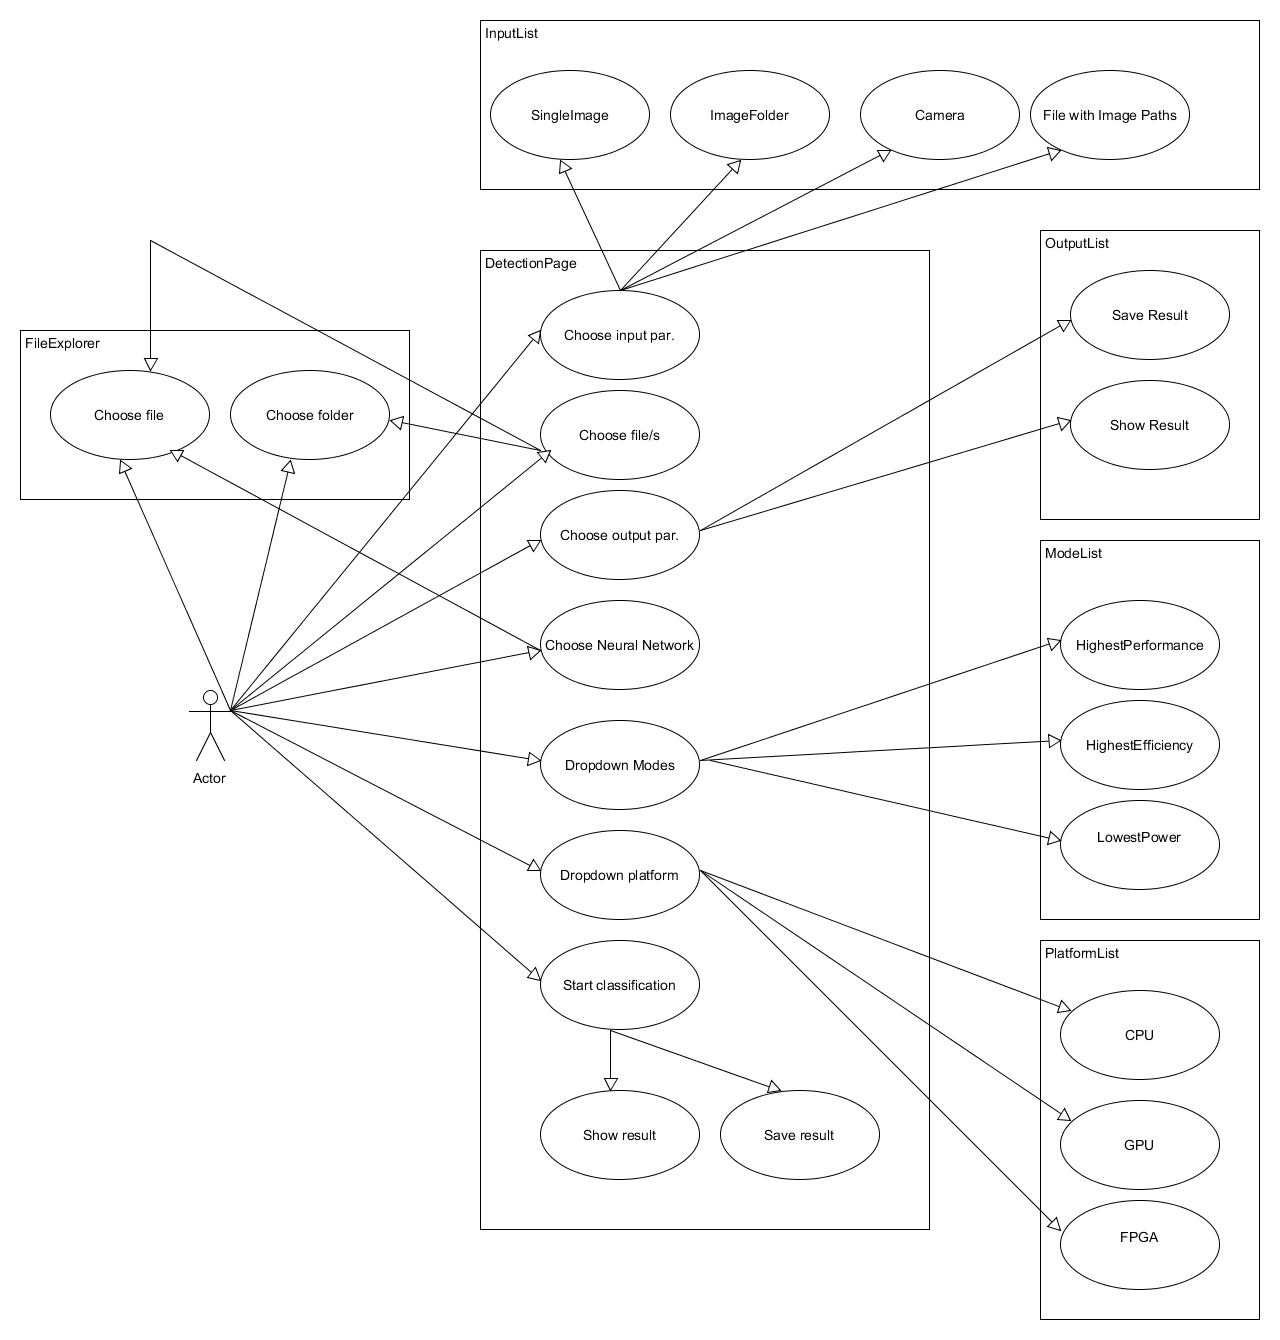
\includegraphics[width=\textwidth]{ClassificationUsecase}
\caption{Usecase of the \gls{image classification} page}
\end{figure}
\newpage
\subsubsection{Training page}
\begin{figure}[htb!]
\centering
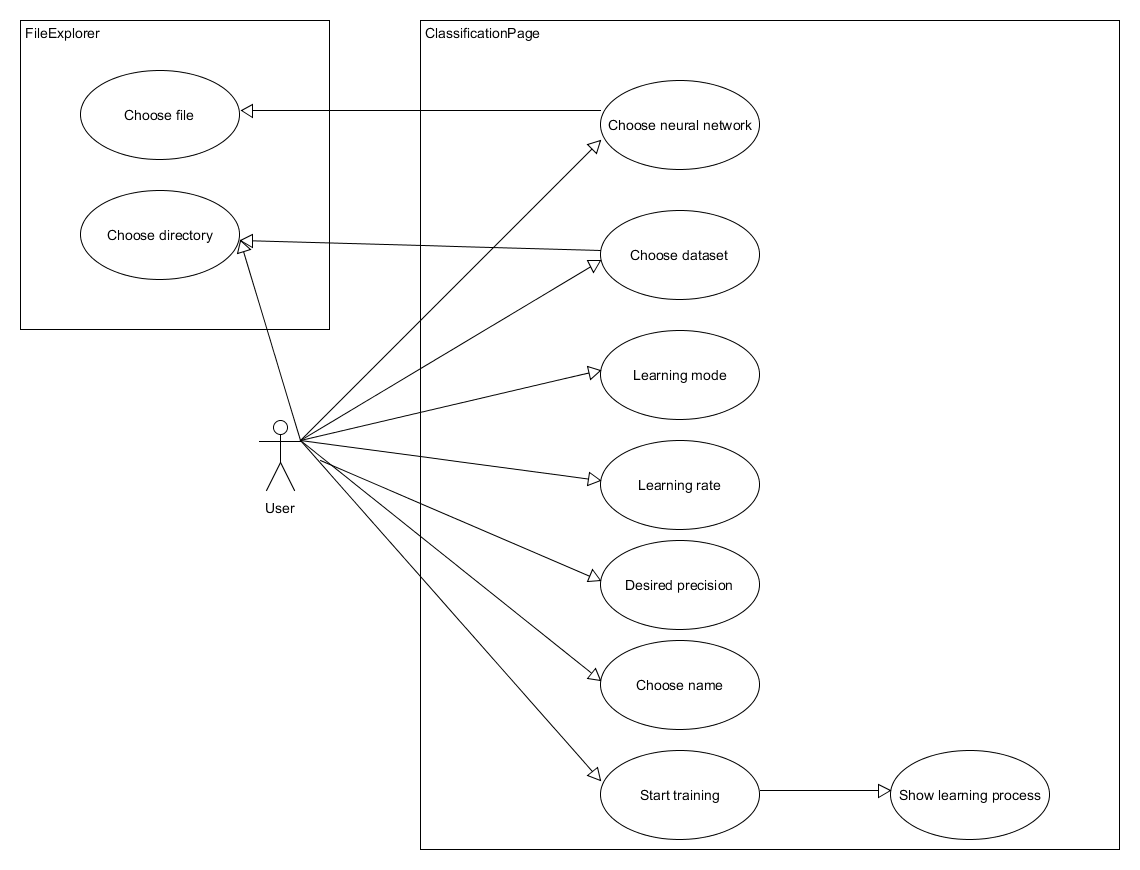
\includegraphics[width=\textwidth]{TrainUsecase}
\caption{Usecase of the trainingspage}
\end{figure}
\clearpage
\subsubsection{Image detection page}
\begin{figure}[htb!]
\centering
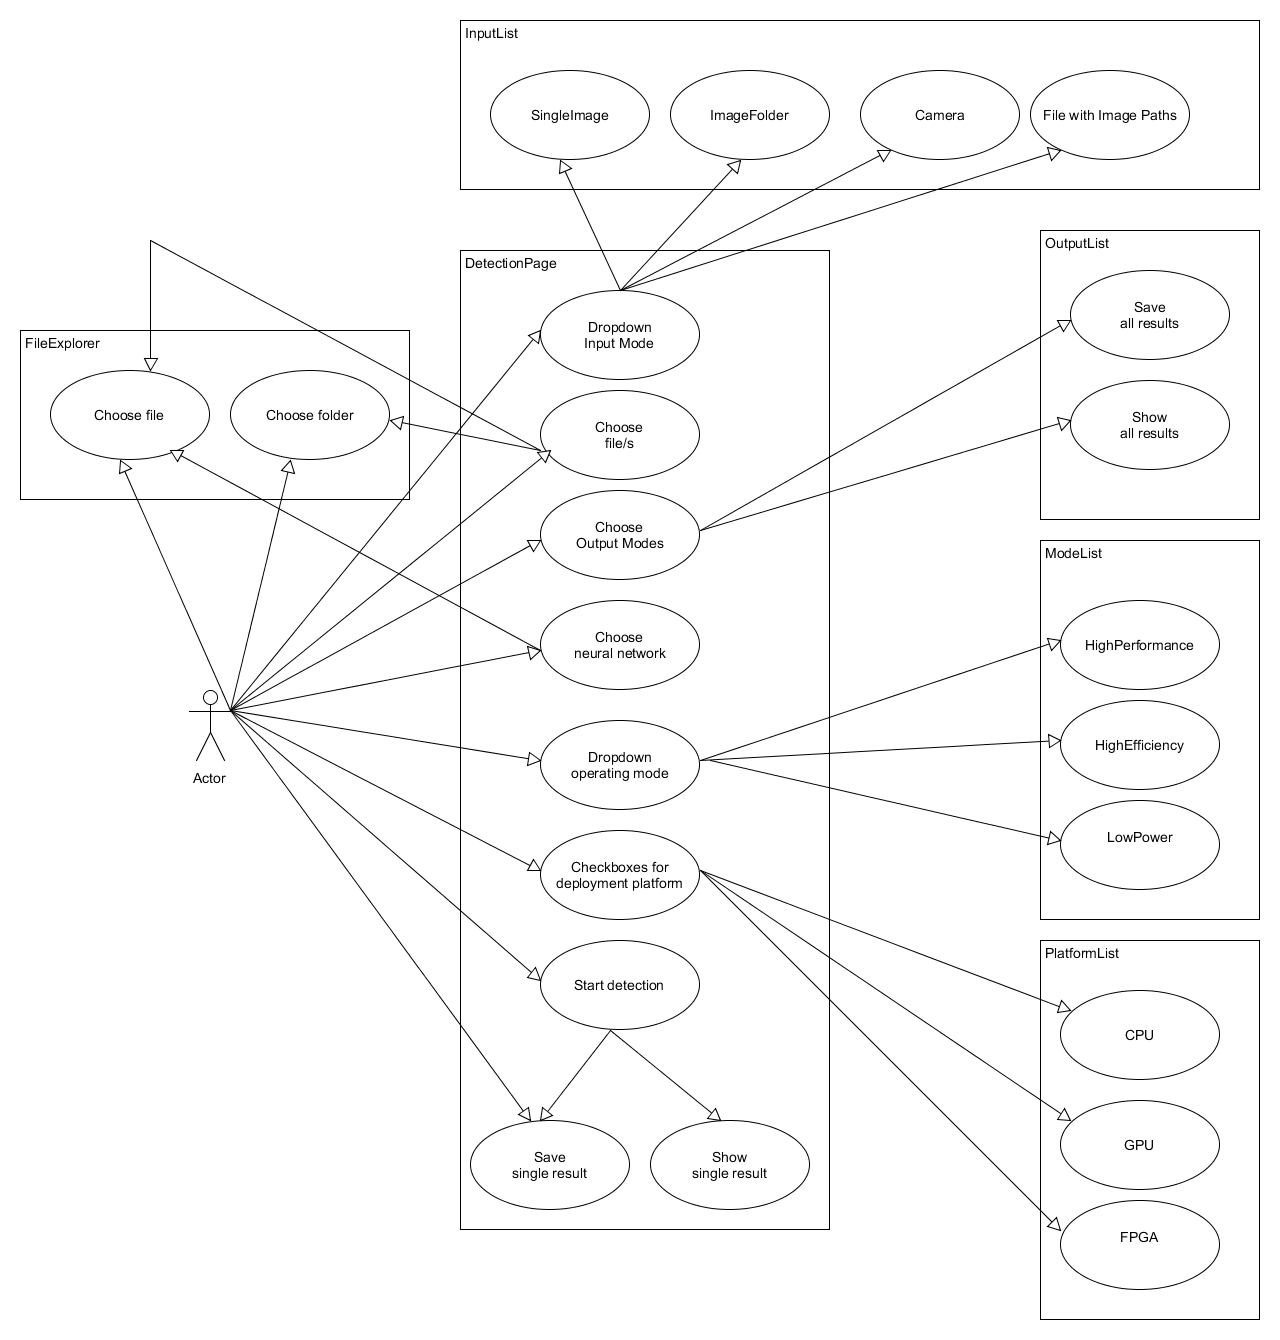
\includegraphics[width=\textwidth]{objectDetectionUsecase}
\caption{Usecase of the image detection page}
\end{figure}
\newpage
\subsubsection{Show topology page}
\begin{figure}[htb!]
\centering
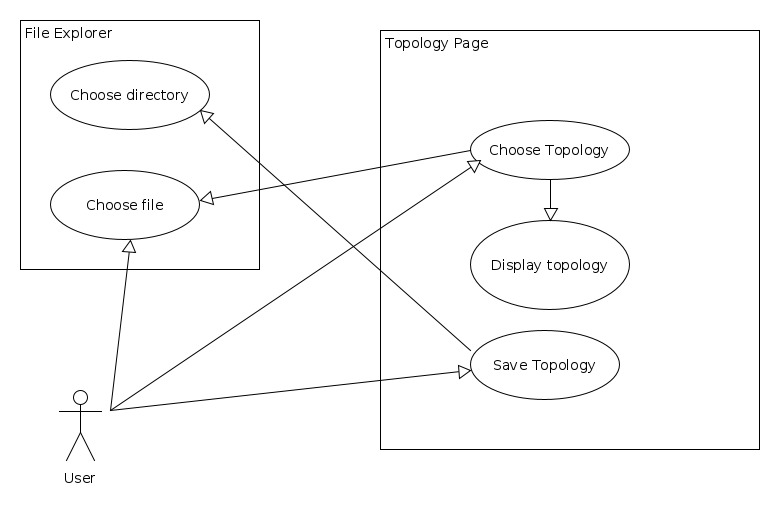
\includegraphics[width=\textwidth]{ShowTopoUsecase}
\caption{Usecase of the image classification page}
\end{figure}
\newpage

\subsection{GUI}
\begin{figure}[htb!]\centering
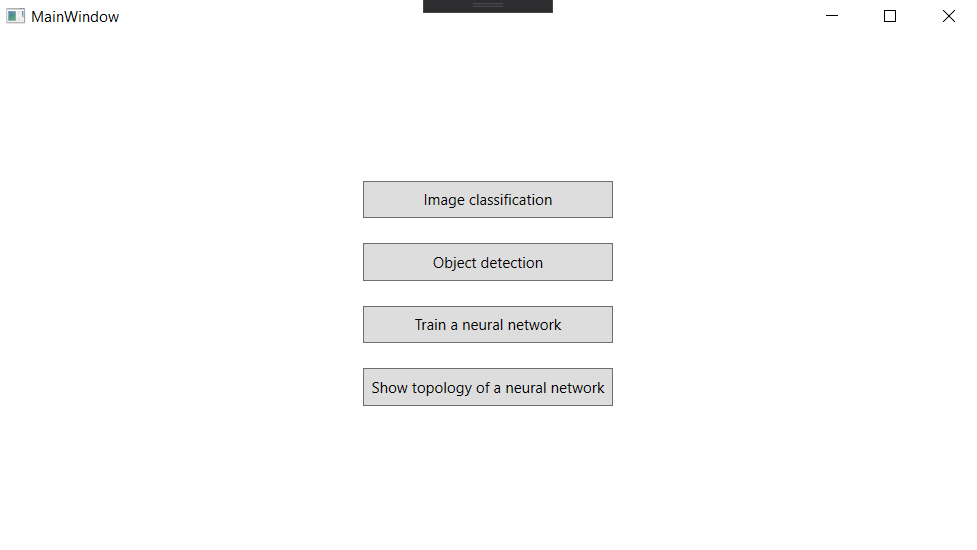
\includegraphics[width=\textwidth]{MainPageGUI}
\caption{Main page of our software}
\end{figure}
\begin{figure}[htb!]\centering
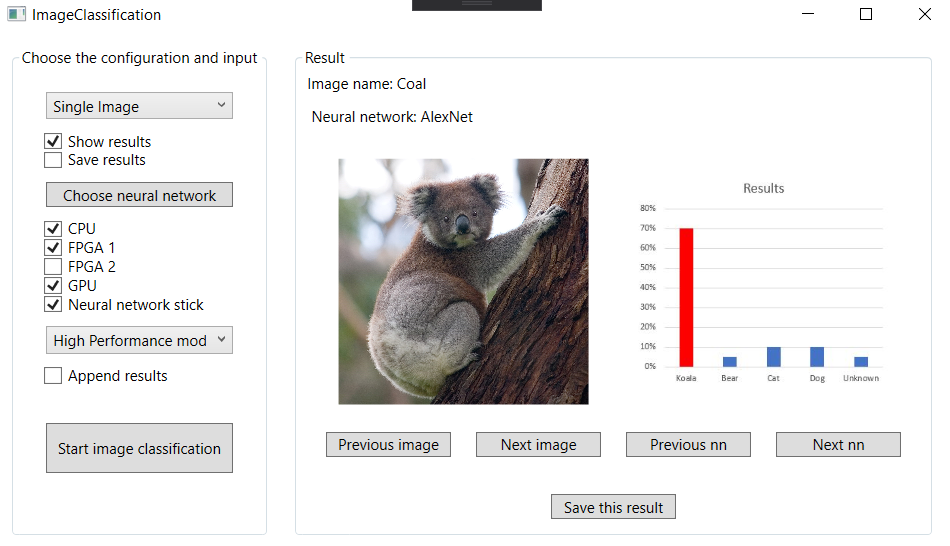
\includegraphics[width=\textwidth]{ImageClassificationGUI}
\caption{\gls{image classification} page of our software}
\end{figure}
\begin{figure}[htb!]\centering
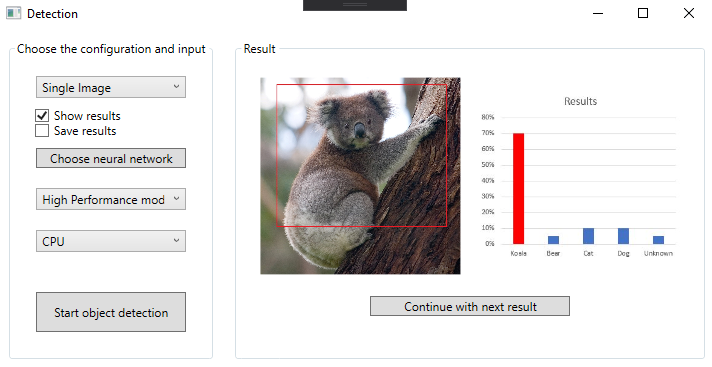
\includegraphics[width=\textwidth]{DetectionGUI}
\caption{Object detection page of our software}
\end{figure}
\begin{figure}[htb!]\centering
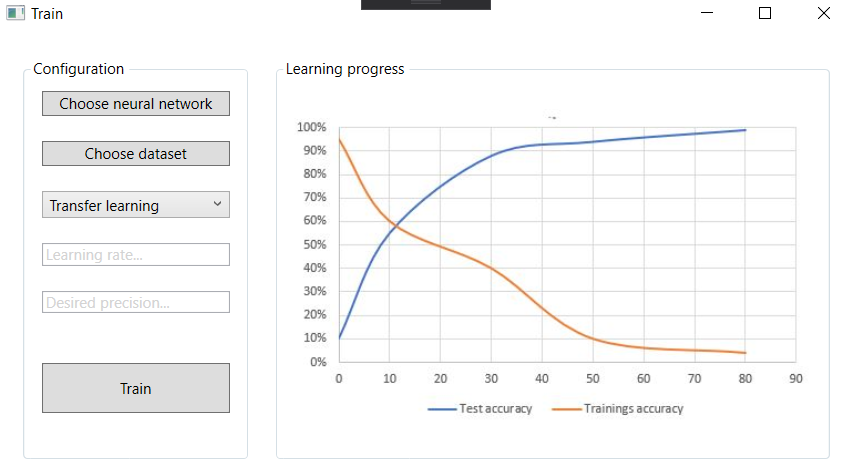
\includegraphics[width=\textwidth]{TrainGUI}
\caption{Training page of our software}
\end{figure}
\begin{figure}[htb!]
\centering
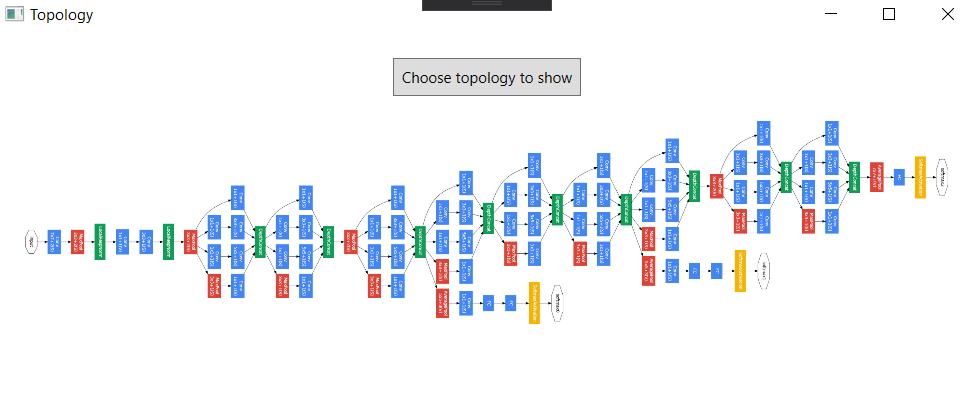
\includegraphics[width=\textwidth]{TopoGUI}
\caption{Page which shows the topology of a selected \gls{nn} of our software}
\end{figure}
\clearpage

\section{Stage responsibilities}
\begin{tabular}{p{4cm}p{8cm}}
\textbf{Requirements:} & Paul Stangel\\
\textbf{Design:} & Johannes Häring\\
\textbf{Implementation:} & Manuel Drehwald\\
\textbf{Quality insurance:}& Stefani Guneshka\\
\textbf{Deployment:} & Dimitar Dimitrov
\end{tabular}

\section{Quality requirements}
\begin{tabular}{|p{3cm}|c|c|c|c|}
\hline
\textbf{Name} & \textbf{Very relevant} & \textbf{Relevant} & \textbf{Less relevant} & \textbf{Not relevant}\\
\hline
Failure tolerance & X & & & \\
\hline
Security & & & & X \\
\hline
Usability & & X & & \\
\hline
Time requirement classification& X & & &\\
\hline
Time requirement detection& & X & &\\
\hline
Extendability & X & & &\\
\hline
\end{tabular}
\clearpage

\printnoidxglossaries
\end{document}

